\documentclass[a4paper,12pt]{article}
\usepackage[english]{babel}
\usepackage{graphicx}
\usepackage{tikz}
\usepackage{wrapfig}
\usepackage{array}
\usepackage{color} 
\usepackage{hyperref}
\usepackage{enumitem}
\usepackage[normalem]{ulem}
\usepackage[font=small,labelfont=bf]{caption}
\usepackage{tcolorbox}
\hypersetup{
    colorlinks,
    citecolor=black,
    filecolor=black,
    linkcolor=black,
    urlcolor=black
}
\usepackage{changepage}
\addto{\captionsenglish}{\renewcommand{\refname}{}}

\begin{document}

\title{%
  Group Project Part 2 - MongoDB \\
  \large of Systems and Methods for Big
    and Unstructured Data Course \\(SMBUD)\\
    held by\\ Brambilla Marco\\ Tocchetti Andrea \\
  \vspace{5mm}
  \Large \textbf{Group 14}}
\author{Banfi Federico\\
  \texttt{10581441}
  \and
  Carotenuto Alessandro\\
  \texttt{10803080}
  \and
  Donati Riccardo\\
  \texttt{10669618}
  \and
  Mornatta Davide\\
  \texttt{10657647}
  \and
  Zancani Lea\\
  \texttt{10608972}}
\date{Academic year 2021/2022}
\maketitle
\begin{center}
  \includegraphics[width=4cm]{polilogo.png}\\
\end{center}
\newpage
\tableofcontents
\newpage
\section{Problem Specification}
\paragraph{}During the sanitary emergency due to the Covid-19 pandemic, many programs and applications developed thanks to the use of Big Data proved to be particularly effective in different settings and scenarios, such as the hospital administration, the hospitalizations organization or the analysis of data relating to various clinical cases. Among the various areas that have been supported by these technologies there is also that which concerns the tracking of populations belonging to a given geographical area and the collection of all information regarding the tests carried out and the vaccination status. \par
Our project aims to create an information system suitable for this specific use case and to do this it is necessary to design a database that allows us to store large amounts of data derived from heterogeneous sources and to carry out targeted queries useful for different purposes. The NOSQL document-based approach, known for being based on managing data saved in JSON-like documents, is the optimal one in this case and MongoDB is the open source database management software that is best suited to accomplish this task thanks to the considerable scalability guaranteed by the automatic data sharding and ease of use thanks to the dynamic schemes developed starting from the archived documents.
\section{Hypotheses}
\paragraph{} During the design phase,some considerations were made regarding how to structure and implement the database to obtain a solution that was effective and performing but at the same time consistent with the real current scenarios. First of all, two types of documents have been created: Certification and AuthorizedBody; the first represents a sort of ”medical chart” containing the following fundamental information for each individual:
  \begin{enumerate}[noitemsep]
    \item list of tests she/he has undergone,
    \item list of vaccine doses that have been administered,
    \item personal details (such as name, surname, date of birth, etc.),
    \item one or more emergency contacts to call in case of need.
   \end{enumerate}
Within the documents stored in the database for each of these four fields, subfields have been provided (as shown in the \texttt{"jsonSchema.json"} file into the \texttt{"documents"} folder) that allow you to manage the various data with MongoDB in order to execute specific queries and commands. \par
The second document contains details related to Authorized Bodies, i.e. institutional places where it is possible to get vaccinated and/or where one can undergo a test, the fields are based on specific assumptions about where these places are located and the healthcare personnel working there. \par
At last, in order to record a greater number of elements to be processed within the dataset, while ensuring the meaningfulness and consistency of the information stored, some assumptions and limitations have been established in the creation of the data managed by the database, therefore:
  \begin{itemize}[noitemsep]
    \item[-] each Authorized Body is associated with a document identified by a unique ID, which is directly referred to in the test/vaccine lists of the Certification document;
    \item[-] each test/vaccine was associated with only one member of the healthcare personnel who represents a sort of ”responsible” for that given administration;
    \item[-] for the sake of simplicity in data management, it was decided that for each Authorized Body there should be a list consisting of at most 5 members of the healthcare personnel, ”responsible” for the various tests/vaccines to which they are associated;
    \item[-] each person can come from any Italian location, but only Authorized Bodies belonging to the city of Milan with the relative coordinates have been examined for the purpose of performing more in-depth analysis on the data;
	\item[-] vaccines were administered throughout the last year while tests during the last month.
  \end{itemize}
\clearpage
\section{ER Diagram}
\paragraph{}
	\begin{center}
 		\includegraphics[width = 15 cm]{ER_diagram.png}
		\captionof{figure}{E-R Diagram}
	\end{center}
\par Starting from the considerations previously exposed regarding the implementation hypotheses, we have drawn an ER diagram (\textbf{Figure 1}) which includes 7 different entities and 4 many-to-many relationships described below in the logical model: \par
  \begin{itemize}[noitemsep]
   	\item[-]	\textbf{Address}(\underline{Address}, \underline{HouseNumber}, CAP, Latitude, Longitude, Municipality)
	\item[-]	\textbf{AuthorizedBody}\underline{(ID}, Department, Name, Type)
	\item[-]	\textbf{Certification}(\underline{ID},\dashuline{Person.CF})
	\item[-]	\textbf{HealthcarePersonnel}(\underline{CF}, Birthdate, Cellphone, Name, Sex, Surname)
	\item[-]	\textbf{Person}(\underline{CF}, Birthdate, Cellphone, Name, Sex, Surname)
	\item[-]	\textbf{Test}(\underline{ID}, Datetime, Result, Type)
	\item[-]	\textbf{Vaccination}(\underline{ID}, Datetime, Dose, Type)
\item[-]	\textbf{AttendsTest}(\underline{HealthcarePersonnel.CF}, \underline{Test.ID})	
	\item[-]	\textbf{AttendsVaccination}(\underline{HealthcarePersonnel.CF}, \underline{Vaccition.ID})
	\item[-]	\textbf{Contact}(\underline{Certification.ID}, \underline{Person.CF})
	\item[-]	\textbf{WorksIn}(\underline{AuthorizedBody.ID}, \underline{HealthcarePersonnel.CF})
  \end{itemize} \par
The \textbf{Person} entity describes each individual and their personal data, \textbf{HealthcarePersonnel} is a specialization of \textbf{Person} and includes all the people (doctors, nurses, pharmacists, etc.) who work (as indicated by the many-to-many \textbf{WorksIn} relationship) at an \textbf{AuthorizedBody}. Both the \textbf{Test} and \textbf{Vaccination} entities are linked to \textbf{HealthcarePersonnel} by the many-to-many \textbf{AttendsTest} and \textbf{AttendsVaccination} relationships, while the link with \textbf{AuthorizedBody} is given by the one-to-many \textbf{AdministersTest} and \textbf{AdministersVaccination}. Each \textbf{Person} can have one and only one (one-to-one relationship \textbf{Has}) \textbf{Certification}, that contains information regarding how many and which tests a person has undergone and whether or not he has received one or more doses of the vaccine, in fact, \textbf{Certification} is in a one-to-many relationship with both \textbf{Test} and \textbf{Vaccination}, through \textbf{IncludesTest} and \textbf{IncludesVaccination}, respectively. Furthermore, each \textbf{Certification} must also include for each \textbf{Person} a sort of "emergency contact" with its details as evidenced by the many-to-many \textbf{Contact} relationship. Finally, to save information relating to the geographical location of persons and authorized bodies, an \textbf{Address} entity was added with specific attributes, connected to \textbf{Person} and \textbf{AuthorizedBody} respectively by the one-to-many \textbf{LivesIn} and \textbf{In} relationships.
\section{Dataset Description}
\paragraph{} Before starting to execute queries and commands based on the design choices that are previously established to define the database structure, it was necessary to generate some sample datasets so that it was possible to work on realistic data during the development and testing phases of the
developed features. \par
There are 2 datasets and they follow the characteristics of the documentary approach, in fact, they represent the Certification and Vaccination documents with the various fields and subfields that trace the structure of the tables expressed in the ER model, they were generated randomly through scripts in Python and were finally saved in .csv format (you can find them into the folder \texttt{"db"}) in order to facilitate the import into MongoDB, below you can consult a table with some metrics to understand the dimensions of the datasets used.
\begin{center}
\begin{tabular}{|l|l|l|l|}
\hline
Pharmacies & 6 & Tests & 302 \\
\hline
Hospitals & 10 & Certifications & 300 \\
\hline
Vaccination Hubs & 4 & Vaccinations & 365 \\
\hline
Tot Authorized Bodies & 20 & Healthcare Personnel & 56 \\

\hline
\end{tabular}
\end{center}
\section{Queries and Commands}
\paragraph{} The correct functioning of the information system involves the implementation of some essential commands and queries for the database in order to properly support the app and to ensure the right execution of searches among the data available for statistical or practical purposes. \par
\paragraph{} First of all you need to load the .csv files in two separate collections (authorizedBodies and certifications), you can find them following the path \texttt{"db/ab.csv"} and \texttt{"db/certification.csv"}
\paragraph{}When you are importing the data make sure to change the datatypes in:
\begin{itemize}
\item[•] All the dates/datetimes from String to Date
\item[•] In certifications test/vaccine.id\textunderscore authorized\textunderscore body from String to ObjectId
\item[•] In authorizedBodies \textunderscore id from String to ObjectId
\end{itemize}

\subsection{Queries}
\subsubsection{Find all the people with the Reinforced GreenPass}
\paragraph{} This query allows us to find all people in possession of a reinforced greenpass after the latest regulations, that is, all those who have been vaccinated in the last 9 months.
\begin{tcolorbox}[colback=green!5!white,colframe=green!75!black,title=QUERY]
\begin{verbatim}
db.certifications.find({
  "$and":[{"vaccination":{"$exists":true}},
  {"vaccination.datetime":{"$gte":new Date(
            ISODate().getTime() - 1000 * 3600 * 24 * 270)}},
  {"vaccination.datetime":{"$lte":new Date(
            ISODate().getTime())}}]
},{
  "person.name":1,
  "person.surname":1,
  "vaccination":1
})
\end{verbatim}
\end{tcolorbox}
\paragraph{} The output is given by: 
\begin{itemize}[noitemsep]
\item[•] The ObjectId of the certification document
\item[•] The name and the surname of the person 
\item[•] The datetime of the vaccination
\end{itemize}
\begin{tcolorbox}[colback=red!5!white,colframe=red!75!black,title=OUTPUT]
\begin{verbatim}
{ _id: ObjectId("61af82fb2468d4592b37b6ee"),
  person: { name: 'Luca', surname: 'Colombo' },
  vaccination: 
   [ { datetime: 2021-09-07T17:31:42.000Z },
     { datetime: 2021-10-05T17:31:42.000Z } ] }
{ _id: ObjectId("61af82fb2468d4592b37b70e"),
  person: { name: 'Lorenzo Federico Giuseppe', 
            surname: 'Tomasi' },
  vaccination: [ { datetime: 2021-11-14T10:18:51.000Z } ] }
{ _id: ObjectId("61af82fb2468d4592b37b6e9"),
  person: { name: 'Vincenzo', surname: 'Maggiani' },
  vaccination: 
   [ { datetime: 2021-10-23T15:51:37.000Z },
     { datetime: 2021-11-20T16:51:37.000Z } ] }
        . . .
\end{verbatim}
\end{tcolorbox}
\clearpage
\subsubsection{Find the number of vaccinations ordered per month}
\paragraph{} This query allows us to retrieve some statistical data on the number of the vaccinations per month.
\begin{tcolorbox}[colback=green!5!white,colframe=green!75!black,title=QUERY]
\begin{verbatim}
db.certifications.aggregate(
    { $unwind : "$vaccination" }, 
    { $group: {
        _id: {month: { $month: "$vaccination.datetime" },
        year: { $year: "$vaccination.datetime" } },
        count: { $sum: 1 }
    }
    },{
      "$sort":{count:-1}
    }
)
\end{verbatim}
\end{tcolorbox}
\paragraph{} The output is given by: 
\begin{itemize}[noitemsep]
\item[•] The count of the vaccinations
\item[•] The months and year
\begin{tcolorbox}[colback=red!5!white,colframe=red!75!black,title=OUTPUT]
\begin{verbatim}
{ _id: { month: 11, year: 2021 }, count: 41 }
{ _id: { month: 2, year: 2021 }, count: 36 }
{ _id: { month: 10, year: 2021 }, count: 36 }
{ _id: { month: 8, year: 2021 }, count: 36 }
{ _id: { month: 4, year: 2021 }, count: 35 }
{ _id: { month: 3, year: 2021 }, count: 32 }
{ _id: { month: 12, year: 2021 }, count: 29 }
{ _id: { month: 5, year: 2021 }, count: 27 }
{ _id: { month: 7, year: 2021 }, count: 27 }
{ _id: { month: 9, year: 2021 }, count: 26 }
{ _id: { month: 1, year: 2021 }, count: 22 }
{ _id: { month: 6, year: 2021 }, count: 14 }
\end{verbatim}
\end{tcolorbox}

\end{itemize}
\subsubsection{Find the age average of unvaccinated people}
\paragraph{} This query also allows us to get a statistical information about the age of the unvaccinated people
\begin{tcolorbox}[colback=green!5!white,colframe=green!75!black,title=QUERY]
\begin{verbatim}
db.certifications.aggregate([
    { $match : { 
      "person.birthdate" : { $exists : true},
      "vaccine":{"$exists":false}
    } },
    { $project : {"ageInMillis" : {$subtract : 
                 [new Date(), "$person.birthdate"] } } }, 
    { $project : {"age" : {$divide : 
                 ["$ageInMillis", 31558464000] }}},
    // take the floor of the previous number:
    { $project : {"age" : {$subtract : ["$age", 
                 {$mod : ["$age",1]}]}}},
    { $group : { _id : true, avgAge : { $avg : "$age"} } },
    { $project: { "avgAge": { $round: ["$avgAge", 2] }}}
])
\end{verbatim}
\end{tcolorbox}
\paragraph{} The output is given by: 
\begin{itemize}
\item[•] The age average
\end{itemize}
\begin{tcolorbox}[colback=red!5!white,colframe=red!75!black,title=OUTPUT]
\begin{verbatim}
{ _id: true, avgAge: 58.14 }
\end{verbatim}
\end{tcolorbox}

\subsubsection{Find all currently infected people}
\paragraph{} This query allows us to find people currently infected, i.e. those whose last test is positive.
\begin{tcolorbox}[colback=green!5!white,colframe=green!75!black,title=QUERY]
\begin{verbatim}
db.certifications.aggregate([
  {$addFields : {test : {$reduce : {
        input : "$test", 
        initialValue : {datetime : 
             new ISODate('2000-01-01T00:00:00')}, 
        in : {$cond: [{$gte : ["$$this.datetime", 
            "$$value.datetime"]},"$$this", "$$value"]}}
    }}},
     { $match:{"test.result":"Positive"}},
     {$project:{
           "person.name":"$person.name",
           "person.surname":"$person.surname",
           "person.codice_fiscale":"$person.codice_fiscale",
     }}
])
\end{verbatim}
\end{tcolorbox}
\paragraph{} The output is given by: 
\begin{itemize}[noitemsep]
\item[•] The ObjectId of the certification document
\item[•] The name and surname of the person
\item[•] The CF of the person
\end{itemize}
\begin{tcolorbox}[colback=red!5!white,colframe=red!75!black,title=OUTPUT]
\begin{verbatim}
{ _id: ObjectId("61af82fb2468d4592b37b71e"),
  person: 
   { name: 'Adele',
     surname: 'Mantovani',
     codice_fiscale: 'MNTDLA62D60C059I' } }
{ _id: ObjectId("61af82fb2468d4592b37b71b"),
  person: 
   { name: 'Ferruccio',
     surname: 'Meloni',
     codice_fiscale: 'MLNFRC61D17B246A' } }
{ _id: ObjectId("61af82fb2468d4592b37b7ab"),
  person: 
   { name: 'Riccardo',
     surname: 'Brumat',
     codice_fiscale: 'BRMRCR65T22F356R' } }
\end{verbatim}
\end{tcolorbox}


\subsubsection{Find the number of tests per authorized body (JOIN) }
\paragraph{} This query allows us to find the number of tests that each authorized body did, in this query we use the JOIN of the two document in order to retrieve the name and the type of the authorized body starting from the id in the certification document. 
\paragraph{}MongoDB is not optimized to perform this type of operation like relational databases, so the query is optimized to perform the join on as few elements as possible grouping the tests in pipeline before the join.

\begin{tcolorbox}[colback=green!5!white,colframe=green!75!black,title=QUERY]
\begin{verbatim}
db.certifications.aggregate([
  { $unwind : "$test" },
  {$group:{
    _id:"$test.id_authorized_body",
    count:{$sum:1}
  }},
  {
    "$lookup": {
        "from": "authorizedBodies",
       "localField": "_id",
        "foreignField": "_id",
        "as": "authorizedBodyInfo"
        }
  },
  {
    "$project":{_id:0,count:1,
    "authorizedBodyInfo.name":"$authorizedBodyInfo.name",
    "authorizedBodyInfo.type":"$authorizedBodyInfo.type"
    }
  }
  ])
\end{verbatim}
\end{tcolorbox}

\paragraph{} The output is given by: 
\begin{itemize}[noitemsep]
\item[•] The count of the tests done
\item[•] The name of the authorized body
\item[•] The type of the authorized body
\end{itemize}

\begin{tcolorbox}[colback=red!5!white,colframe=red!75!black,title=OUTPUT]
\begin{verbatim}
{ count: 17,
  authorizedBodyInfo: [ { name: [ 'Policlinico' ],
                          type: [ 'Hospital' ] } ] }
{ count: 21,
  authorizedBodyInfo: [ { name: [ 'Auxologico San Luca' ], 
                          type: [ 'Hospital' ] } ] }
{ count: 25,
  authorizedBodyInfo: [ { name: [ 'San Raffaele' ],
                          type: [ 'Hospital' ] } ] }
{ count: 19,
  authorizedBodyInfo: [ { name: [ 'San Paolo' ], 
                          type: [ 'Hospital' ] } ] }
{ count: 26,
  authorizedBodyInfo: [ { name: [ 'San Giuseppe' ], 
                          type: [ 'Hospital' ] } ] }
{ count: 15,
  authorizedBodyInfo: [ { name: [ 'Ospedale Fiera' ], 
                          type: [ 'Hospital' ] } ] }
        . . .
\end{verbatim}
\end{tcolorbox}


\subsection{Commands}
\subsubsection{Insert a new Authorized Body (CREATE)}
\paragraph{} In this command we insert in the authorizedBodies collection a new document.

\begin{tcolorbox}[colback=orange!5!white,colframe=orange!75!black,title=COMMAND]
\begin{verbatim}
db.authorizedBodies.insertOne({
  "address":{
    "address":"Via Roma",
    "cap":"24030",
    "geopoint":"45.0000 9.0000",
    "house":"13b",
    "municipality":"Bergamo",
  },
  "department":"covid test",
  "name":"Farmacia Comunale",
  "type":"pharmacy",
  "healthcarePersonnel":[
    {
      "cellphone":"+393476574382",
      "codice_fiscale":"DNTHGB87P15G764J",
      "name":"Carlo",
      "role":"pharmacist",
      "surname":"Merlutti",
    }
  ]
})
\end{verbatim}
\end{tcolorbox}

\subsubsection{Insert a test in a Certification (UPDATE) }
\paragraph{} In this command we add to a given certification (via ObjectId) a new test as a subdocument in the ArrayList field test.
\begin{tcolorbox}[colback=orange!5!white,colframe=orange!75!black,title=COMMAND]
\begin{verbatim}
db.certifications.updateOne({
  "_id":ObjectId('61af82fb2468d4592b37b70e')
},{
  "$push":{
    "test":{
      "$each":[{
        "datetime":ISODate('2021-12-08T16:20:00'),
        "healthcarePersonnel":{
          "codice_fiscale":"PLCLRT48C02C224Y",
          "name":"Alberto Christian",
          "surname":"Paolucci"
        },
        "id_authorized_body":
                ObjectId('61acd3e25ca7e964a122def1'),
        "result":"Positive",
        "type":"Molecular"
      }]
    }
  }
})
\end{verbatim}
\end{tcolorbox}


\subsubsection{Delete all the Authorized Bodies that test and are pharmacies (DELETE)}
\paragraph{} In this command we simulate a change of regulations where the pharmacies can no longer test people and therefore we delete this kind of authorized body from the collection.
\begin{tcolorbox}[colback=orange!5!white,colframe=orange!75!black,title=COMMAND]
\begin{verbatim}
db.authorizedBodies.deleteMany({
  "$and":[
    {"type":"pharmacy"},
    {"department":"covid test"}]
})

\end{verbatim}
\end{tcolorbox}
\clearpage
\section{UI Description \& User Guide}
\subsection{UI Description}
\paragraph{}To conclude our project, a simple application connected to the database has been developed, the programming language chosen to write the code is Python which has proved to be particularly useful and versatile thanks above all to the considerable number of libraries made available to developers, including: \emph{PySimpleGUI}, which allows you to create essential and user-friendly graphical interfaces, \emph{PyMongo}, the official MongoDB Python driver for with the database, and \emph{pandas} to manage the analysis and manipulation of data, these libraries are all listed in the \texttt{"requirements.txt"} file in the folder \texttt{"app"}. \par
\begin{center}
 		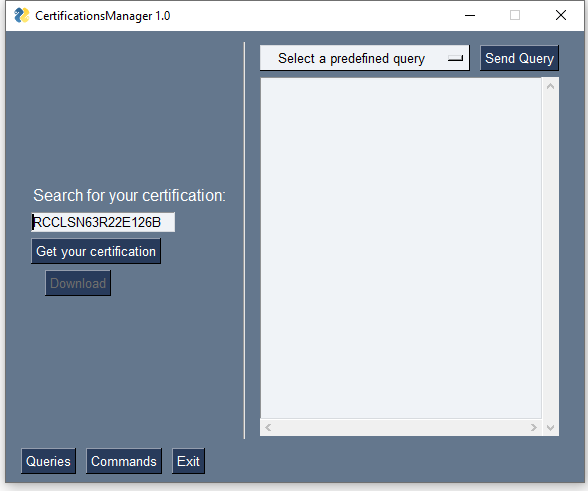
\includegraphics[width = 13 cm]{homepage.png}
		\captionof{figure}{Homepage of CertificationManager 1.0}
\end{center}
\clearpage
\textbf{Figure 2} shows the homepage of the \emph{CertificationsManager 1.0} app, the screen is divided into two side sections: on the left you can obtain your certification starting from your own social security number (if the certification is already present in the database, the "Download" button will be activated and it will be possible to download it \textbf{Figure 3}), on the right you can run a query choosing from the 5 defined and described in Chapter 5 of the report (\textbf{Figure 4}). \par

\begin{center}
 		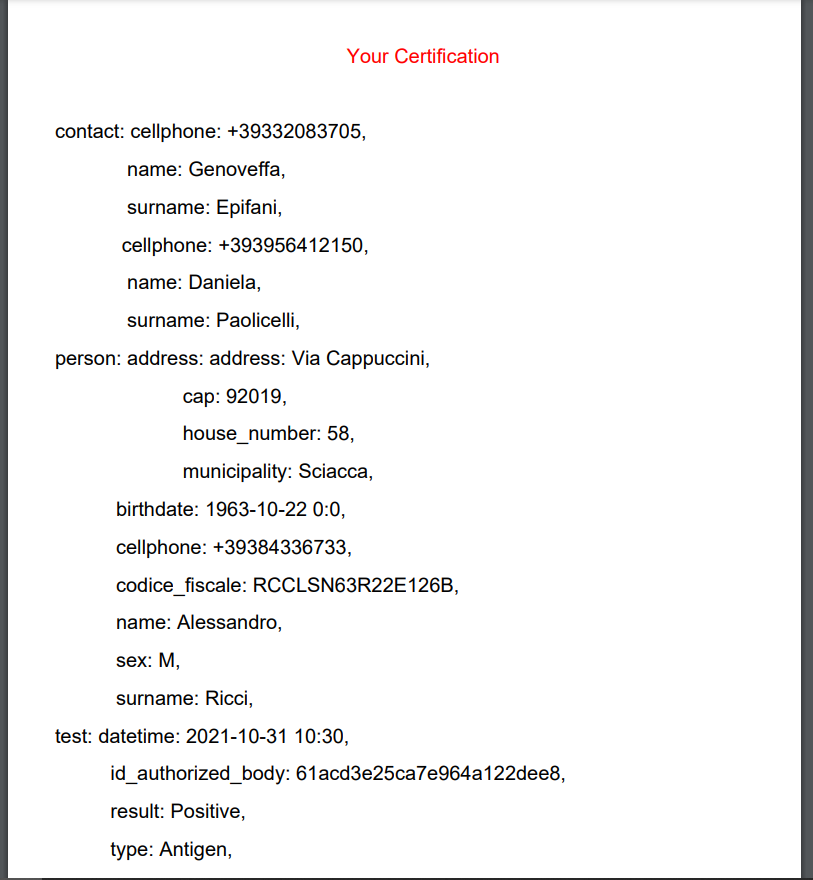
\includegraphics[width = 13 cm]{certification.png}
		\captionof{figure}{A sample certification retrieved from the DB}
\end{center}
\begin{center}
 		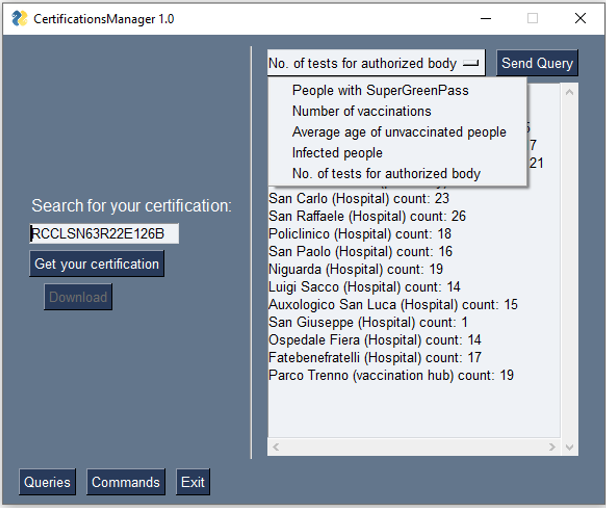
\includegraphics[width = 13 cm]{querylist.png}
		\captionof{figure}{The of the queries implemented into the app}
\end{center}
		
Finally, as shown in \textbf{Figure 5}, it is possible to execute some of the commands already presented in Chapter 5 by reaching the appropriate section of the application by means of the \texttt{"Commands"} button in the lower left corner of the main screen. One of the executable commands allows you to create and add new tests to the certification of a person  by indicating him/her social security numbers, the date and time, the test type and the result.\par
\begin{center}
 		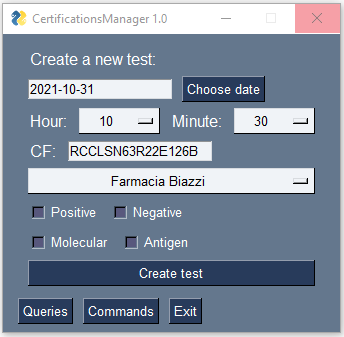
\includegraphics[width = 8 cm]{commands.png}
		\captionof{figure}{The create test command window}
\end{center}
\subsection{User Guide}
\paragraph{}
In order to run the app it is necessary to verify some requirements and to perform some actions:
  \begin{itemize}[noitemsep]
   \item[-] At first you have to check if you have the right Python version installed by using the command: \texttt{python --version}, if not you could download it from the official website: https://www.python.org/ 
   \item[-] Install the required packages (from the \texttt{app} folder): \texttt{pip install -r requirements.txt}
   \item[-] In order to set up MongoDB you have to:
  	\begin{enumerate}[noitemsep]
  		\item Log into your account
  		\item After creating a new Cluster, click on  \texttt{Connect} on the cluster
		\item Then choose as connection method \texttt{Connect your application}
		\item Select your driver \texttt{Python} and version \texttt{3.6 or later}
		\item Add your connection string into the application code by copying the link that has been generated
		\item Replace the link obtained in line 159 of the app.py source code, remembering to replace \texttt{<password>} and \texttt{<myFirstDatabase>} respectively with the user password and name of the database that the connection will use by default
		\item Create the database with \texttt{database name = smbud\_data} and the collections with \texttt{collection name = certifications} and \texttt{collection name = authorizedBodies}
		\item To populate the collections, import respectively the \texttt{certifications.csv} and \texttt{ab.csv} files present in the \texttt{db} folder of the repo and modify all dates with type \texttt{date} and all ids with type \texttt{objectID}

  	\end{enumerate}
	\item[-] Finally make it run by navigating to the folder where this repository has been cloned, then into \texttt{app} folder and run: \texttt{python} \texttt{app.py}
	\item[-] From there you can execute queries about the collected data.
  \end{itemize}

\newpage
\section{References \& Sources}
  \begin{thebibliography}{9}
    \bibitem{} Course Slides
    \bibitem{} https://pysimplegui.readthedocs.io/en/latest/call\%20reference/
    \bibitem{} https://docs.mongodb.com/manual/
    \bibitem{} https://pymongo.readthedocs.io/en/stable/
    \bibitem{} http://iniball.altervista.org/Software/ProgER
    \bibitem{} https://pandas.pydata.org/docs/
  \end{thebibliography}
\end{document}
